\section{Konzeption}

\subsection{Festlegung der Systemanforderungen}

Die grundlegende Anforderung an diese Studienarbeit war es, ein Sprecheridentifikationssystem zu entwickeln, welches über eine Webapplikation bedient werden kann.
Da diese Anforderungsbeschreibung noch viel Spielraum über den Funktionsumfang dieses Systems lässt, werden in diesem Kapitel die Anforderungen an das System genauer spezifiziert.


\begin{itemize}
    \item Das System soll lediglich ein Demo-System darstellen, welches die Machbarkeit eines text-unabhängigen Sprecheridentifikationssystems aufzeigt. Es soll nicht in einem produktiven Umfeld eingesetzt werden können.
    \item Der Datensatz für das System ist zu Begin festgelegt. Das heißt, es werden nur bereits bekannte Sprecher identifiziert. Zudem können keine neuen Sprecher registriert werden, wodurch das Sprecheridentifikationssystem keine dynamische Erweiterung um Sprecher bereitstellen muss.
    \item Das System beschränkt sich auf das Identifizieren eines Sprechers unter 20 Sprechern.
    \item Zur Authentifizierung eines Sprechers wird ein 20 sekündiger Audio-Clip an das System übermittelt. Der Audio-Clip ist dem System bisher unbekannt, aber in gleichen Bedingungen aufgenommen, wie die bekannten Clips.
    \item Das Sprecheridentifikationssystem sollte Teil des Back-Ends sein. Die Bedienung erfolgt über eine Webapplikation, die mit dem System über eine Schnittstelle kommuniziert.
    \item In der Web-Oberfläche des Demo-Systems soll der zu authentifizierende Sprecher (einer der 20) und ein Verifikations-Clip ausgewählt werden können. Es soll für jeden Sprecher 5 Clips zur Auswahl geben.
    \item So soll der Nutzer des Demo-Systems testen können, was passiert, wenn ein zu dem zu authentifizierenden Sprecher passender bzw. unpassender Verifikations-Clip ins System gegeben wird.
    \item Das System soll dem Nutzer dann Informationen über die Identifikations-Verteilung (zu welchem Sprecher passt der Clip zu welchem Prozentsatz) und den Authentifizierungs-Status (\gqq{erfolgreich}/\gqq{nicht erfolgreich}") als Rückmeldung darstellen.
\end{itemize}

\subsection{Demosystem}
Das Demosystem baut auf dem Versuchssystem auf.
Wie in den Anforderungen beschrieben, ist die Authentifizierung und damit auch das Versuchssystem Teil des Back-Ends.
\begin{figure}
    \centering
    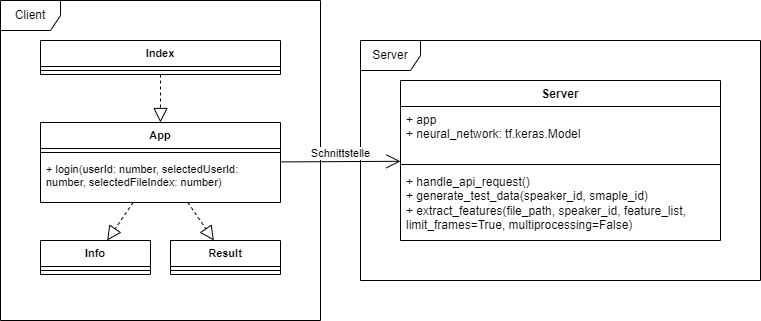
\includegraphics[width=0.8\textwidth, keepaspectratio]{images/Architektur-Demosystem.png}
    \caption{Architektur Demosystem}
    \label{fig:ArchitectureDemoSystem}
\end{figure}
In Abbildung~\ref{fig:ArchitectureDemoSystem} ist die grundlegende Architektur des Demosystems dargestellt.
Diese unterteilt sich in die zwei Elemente: Client (Front-End) und Server (Back-End).

\subsubsection{Server}
Der Server erhält dafür einen eigenen Einstiegspunkt, welcher eine Schnittstelle für den Client bereitstellt.
Gleichzeitig fungiert der Server als Authentifizierungssystem.
Dafür werden die Hauptkomponenten des Versuchssystem (DataSetHandler, AudioPreprocessor und FeatureExtractor) vom Server implementiert.

\begin{figure}
    \centering
    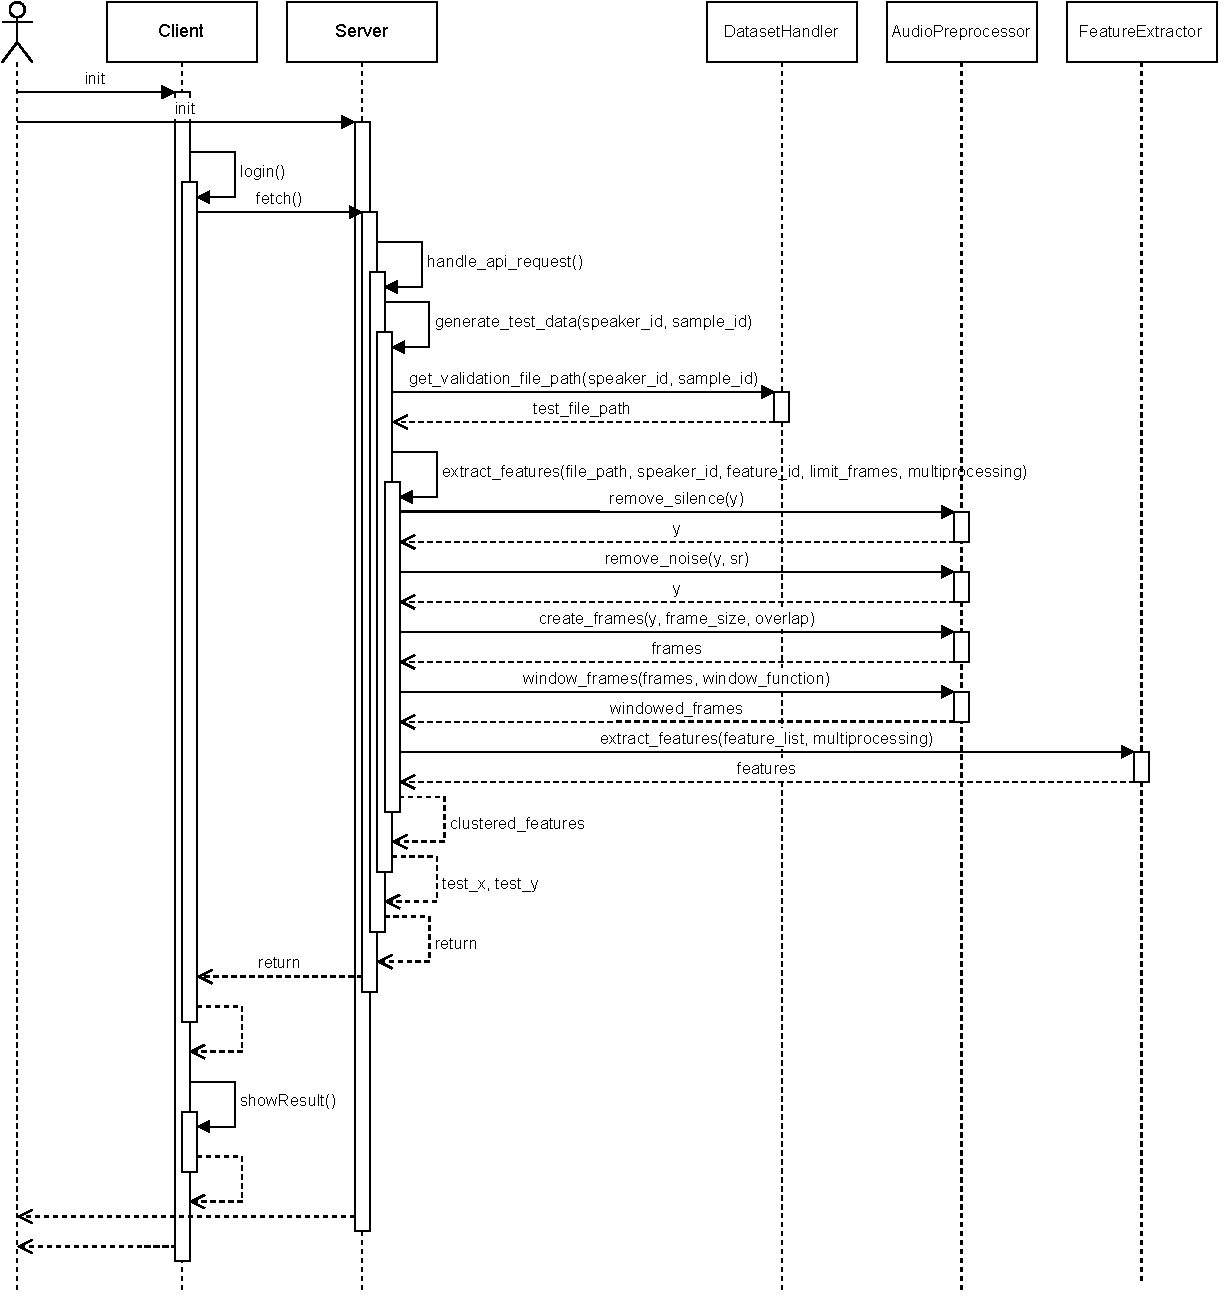
\includegraphics[width=0.8\textwidth, keepaspectratio]{images/SequenzdiagrammClientServer}
    \caption{Sequenzdiagramm handle\_api\_request (Server)}
    \label{fig:SequenceHandleApiRequest}
\end{figure}
Abbildung~\ref{fig:SequenceHandleApiRequest} zeigt den Ablauf der über die Schnittstelle bereitgestellten Authentifizierungsfunktion des Servers als Sequenzdiagramm.
Dabei werden wie in den Anforderungen festgelegt, die Ergebnisse der Authentifizierung an den Client zurückgegeben.

\subsubsection{Client}
Der Client stellt die grafische Oberfläche für den Endnutzer bereit.
Diese untergliedert sich in vier Komponenten.
Index stellt den Einstiegspunkt der Applikation dar.
Dieser implementiert lediglich die App Komponente.

Innerhalb der App Komponente wird nun der allgemeine Login-Prozess dargestellt (vgl. Abbildung~\ref{fig:SequenceHandleApiRequest}).
Die Antwort des Servers wird dabei mittels einer zusätzlichen Komponente (Result) grafisch dargestellt.

Für eine verbesserte Nutzerfreundlichkeit wird zusätzlich eine Info Komponente eingebunden, welche die grundlegende Bedienung und Vorgehensweise des Demosystems erklärt.

\subsubsection{Schnittstellendefinition}
Im Konkreten enthält die Anfrage des Clients die folgenden Informationen:
\begin{itemize}
    \item Zu authentifizierender Sprecher
    \item Index der ausgewählten Sprachdatei
    \item Sprecher der ausgewählten Sprachdatei
\end{itemize}
Die Antwort des Servers beinhaltet die Informationen:
\begin{itemize}
    \item Ermittelte Wahrscheinlichkeit des zu authentifizierenden Sprechers
    \item Authentifizierungsstatus
    \item Ermittelte Wahrscheinlichkeit je Sprecher
\end{itemize}